\chapter{Introduction}


\section{Problem description and motivation}

\subsection{3D arrays}

Sound propagates in 3D: need for 3D mic arrays to capture spatial properties



\subsection{spherical microphone arrays}

\begin{itemize}
  \item even distribution of capsules
  \item mathematical convenience: spherical harmonics
\end{itemize}



\subsection{ambisonics}


advantages on the vr/ar context
\begin{itemize}
  \item device independent
  \item intermediate storage format
  \item signal-independent transformations are easy
  \item de-facto standard for vr
\end{itemize}

\subsection{Current limitations of vr/ar production}


\section{Goals}

Research question: 	How can we exploit the characteristics of ambisonic recordings in order to extract signal-dependent, meaningful information from them? 


\section{Context}
\label{sec:context}

Different levels of applications:

\begin{itemize}
	\item Acoustic Parameter Estimation (low level, audio2data)
	\begin{itemize}
		\item Direction of Arrival estimation
		\item Coherence analysis
		\item Acoustic description (RT60, etc)
		\item Source counting
	\end{itemize}

	\item Signal Enhancement  (high level, audio2audio)
	\begin{itemize}
		\item Source Separation
		\item Dereverberation / denoising
		\item IR estimation
	\end{itemize}

	\item Scene Description (high level, audio2data)
	\begin{itemize}
		\item Event Detection
		\item Acoustic Scene Classification
	\end{itemize}
\end{itemize}

\begin{figure}[hbt]
  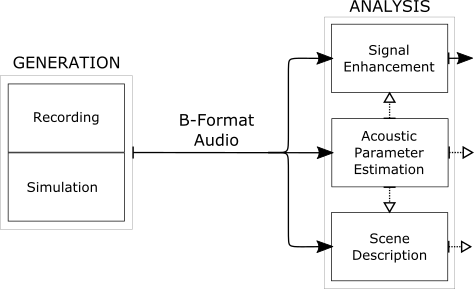
\includegraphics[width=\textwidth]{Figures/Introduction/SCHEME1.png}
  \caption{\todo{todo caption}}
  \label{fig:scheme1}
\end{figure}


\section{Outline and main contributions}

\subsection{Thesis structure}


The present Thesis is organised as follows. 

\textbf{Chapter~\ref{chap:scientific}} introduces the basic concepts that will be developed throughout the Thesis, including spherical harmonics and ambisonics, coherence estimation, parametric analysis or room acoustics. The Chapter also defines the signal models and the mathematical terminology.

Chapters~\ref{chap:rt60}, \ref{chap:coherence} and \ref{chap:seld2019} develop the most significant academic contributions of the Thesis. 
\textbf{Chapter~\ref{chap:rt60}} presents a novel method for blind reverberation time in ambisonic recordings. To the best of our knowledge, this is the first method proposal specifically focusing on that problem.   The method is based on a Multichannel Auto-Regressive model of the late reverberation, which allows for an effective dereverberation of the ambisonic sound scene, and enables computation of the reverberation time from an estimation of the room impulse response. The evaluation metrics show a method performance similar to other state-of-the-art methods. 
\textbf{Chapter~\ref{chap:coherence}} analyses the response of tetrahedral microphone arrays, which are the simplest and most common form of ambisonic microphones, under spherically isotropic sound field. The analysis is performed using both simulated and recorded diffuse field, and the results quantify the differences between ideal and real values under a variety of conditions and estimators.  
In \textbf{Chapter~\ref{chap:seld2019}}, a complete system for Sound Event Localization and Detection of ambisonic sound scenes is described. The algorithm comprises two different parts. First, a parametric analysis is performed on the ambisonic signal. The analysis yields spatial localization and temporal activities of the sound events present in the scene. Then, each of those events is assigned to a class label by means of a deep-learning classifier. The method is able to perform in a similar way to the baseline system, while greatly improving its localization capabilities.

Finally, \textbf{Chapter~\ref{chap:data}} presents some libraries and software utilities developed throughout the Thesis. All the code has been publicly released under open source licenses. The libraries include utilities for the creation of datasets, the storage and exchange of impulse response files in a standard way, and the implementation of convenience tools for acoustic and microphone array signal processing analysis. Although the libraries do not directly involve any scientific contribution, they can be a great help for scientific and innovative purposes; given the industial nature of the candidate's doctoral program, we have considered relevant to include them in the present Thesis. \todo{check}

In order to place the different chapters within the problem context described in Section~\ref{sec:context}, we add to Figure~\ref{fig:scheme1} the Chapter numbers with our contributions, obtaining Figure~\ref{fig:scheme1_numbers}.


\begin{figure}[hbt]
  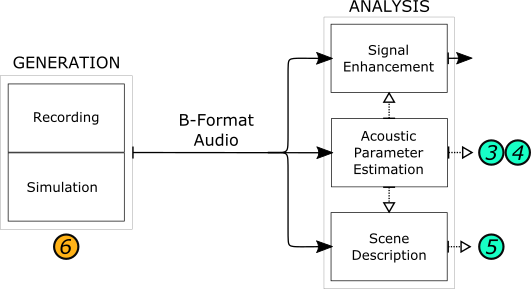
\includegraphics[width=\textwidth]{Figures/Introduction/SCHEME1_NUMBERS.png}
  \caption{\todo{todo caption}}
  \label{fig:scheme1_numbers}
\end{figure}

%\newpage
\subsection{List of Publications}

In the following list we show the main scientific contributions of the Thesis, organised by Chapters:

\begin{itemize}

	\item Chapter 3:\\
	\textbf{"Blind reverberation time estimation from ambisonic recordings"}.
	\underline{A. P\'erez-L\'opez}, A. Politis and E. G\'omez.
	Submitted to \textit{IEEE 22nd International Workshop on Multimedia Signal Processing, 2020.}
	
	\item Chapter 4:\\
	\textbf{"Analysis of spherical isotropic noise fields with an A-Format tetrahedral microphone"}.
	\underline{A. P\'erez-L\'opez} and N. Stefanakis.
	\textit{The Journal of the Acoustical Society of America 146.4 (2019): EL329-EL334.}

	\item Chapter 5:\\
	\textbf{A hybrid parametric-deep learning approach for sound event localization and detection.}
	\underline{A. P\'erez-L\'opez}, E. Fonseca and X. Serra.
	In \textit{Proceedings of the Detection and Classification of Acoustic Scenes and Events 2019 Workshop (DCASE2019)}.
	
	\item Chapter 6:\\
	\textbf{Ambiscaper: A Tool for Automatic Generation and Annotation of Reverberant Ambisonics Sound Scenes}.\\
	\underline{A. P\'erez-L\'opez}.
	In \textit{16th International Workshop on Acoustic Signal Enhancement (IWAENC). IEEE, 2018.}
	
	\textbf{Ambisonics directional room impulse response as a new convention of the spatially oriented format for acoustics.}
	\underline{A. P\'erez-L\'opez} and J. De Muynke.
	In \textit{Audio Engineering Society Convention 144. Audio Engineering Society, 2018.}
	
	\textbf{pysofaconventions, a Python API for SOFA.}
	\underline{A. P\'erez-L\'opez}.
	In \textit{Audio Engineering Society Convention 148. Audio Engineering Society, 2020.}
	
	\textbf{A Python library for Multichannel Acoustic Signal Processing.}
	\underline{A. P\'erez-L\'opez} and A. Politis.
	In \textit{Audio Engineering Society Convention 148. Audio Engineering Society, 2020.}
	
\end{itemize}


Moreover, as a result of the development of the Thesis, the following open-source libraries have been implemented and released. All of them are available through the author's GitHub page, \url{https://github.com/andresperezlopez}: \todo{describir cada uno? con respecto a paper o chapter?}

\begin{itemize}

	\item rt60 estimation: \todo{todo}
	
	\item \href{https://github.com/andresperezlopez/DCASE2019_task3}{DCASE2019\_task3}

	\item \href{https://github.com/andresperezlopez/ambiscaper}{ambiscaper} 
	
	\item \href{https://github.com/andresperezlopez/pysofaconventions}{pysofaconventions}
	
	\item \href{https://github.com/andresperezlopez/masp}{masp: Multichannel Acoustic Signal Processing library}
	
\end{itemize}



